% !TeX spellcheck = en_GB
% !TeX encoding = UTF-8
% !TeX root = ../thesis.tex
\chapter{N-Gram Bug Detection in \scratch{}}\label{chap:methods}
%TODO Unfinished chapter!

\begin{figure}[hbtp]
\centering
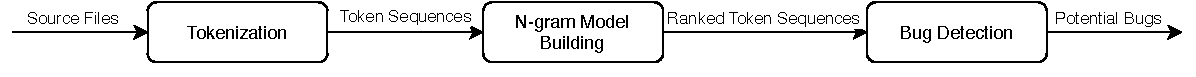
\includegraphics[scale=0.75]{images/Overview.pdf}
\caption{Overview of the n-gram model building process}
\label{fig:overview}
\end{figure}

Figure \ref{fig:overview} visualizes the \ngram{} building process which is explained in this chapter in more detail. In Section~\ref{sec:tokenization} the tokenization process is described with the way the \scratch{} project is parsed and converted into tokens. The next step is to use the created tokens to build the \ngram{} like it is shown in Section~\ref{sec:model}. Finally, bugs can be detected with the help of the calculated model according to Section~\ref{sec:detection}.

\section{Tokenization of \scratch{} Code}\label{sec:tokenization}
In order to build a model, we need to tokenize the \scratch{} project into suitable pieces:

\begin{definition}[Token]\label{def:token}
    %
    ``A token is a single fragment of \scratch{} code that is used to partition code into smaller pieces in order to obtain information about its syntax on a specific granularity level.''
    %
\end{definition}

In order to identify unusual block sequences in a \scratch{} project, each project should be represented in the same form and structure. To visualize a \scratch{} project like in Figure~\ref{fig:ast}, the tokenization process is based on the Abstract Syntax Tree (\AST{}) structure of \litterbox{}. 

\begin{figure}[hbtp]
\centering
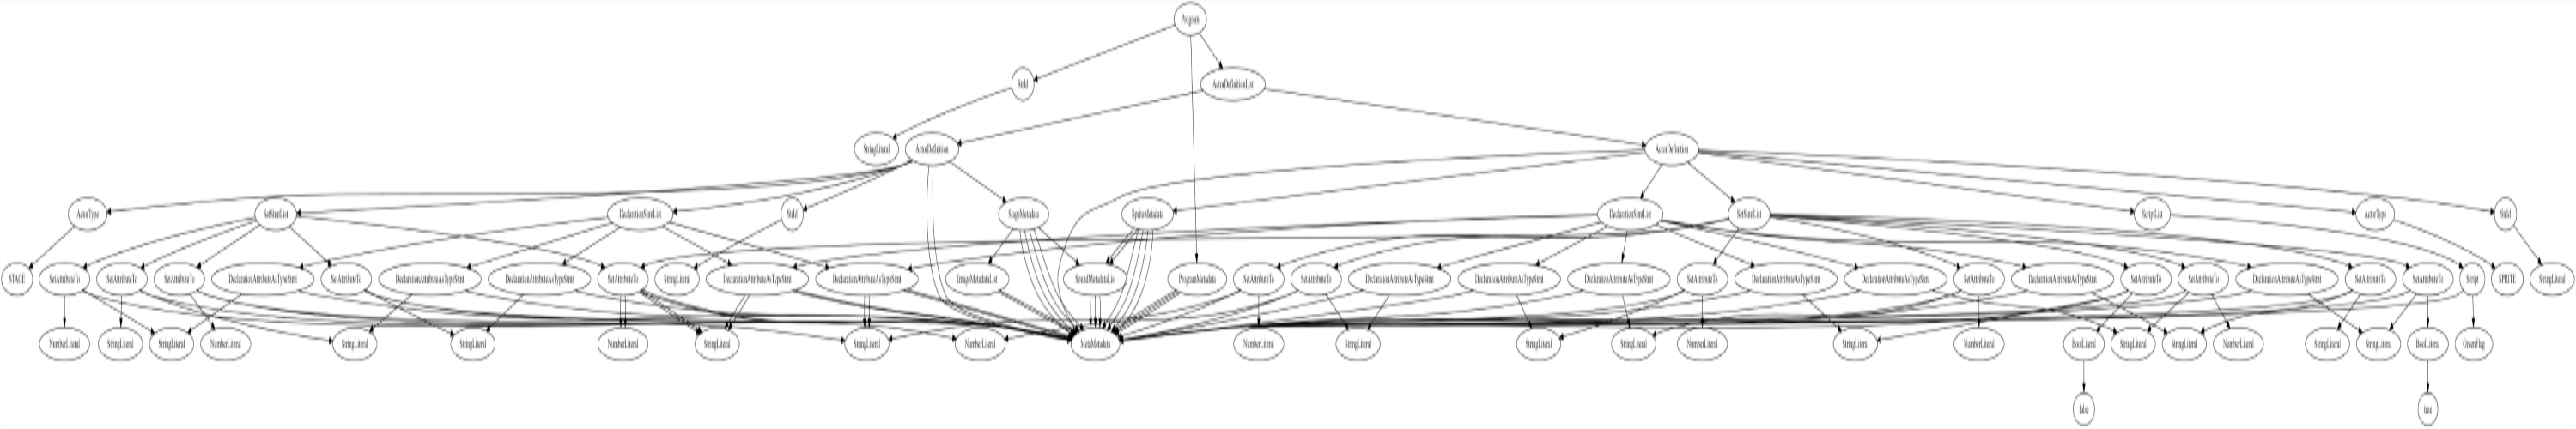
\includegraphics[scale=0.20]{images/AST_example(3).png}
\caption{Example AST structure of a simple \scratch{} project}
\label{fig:ast}
\end{figure}

For a simple \scratch{} project with only one [GreenFlag] block, the tree structure is already pretty big. This is caused by the amount of additional information blocks that are created by the \litterbox{} \AST{} but are not necessary or even part of the essential tokens we need for the \ngram{}. Here in Table~\ref{tab:tokens} is a quick overview of all categories of blocks that are being used for the tokenization and the ones that are excluded in order to keep the n-gram model later as small as possible.   

%TODO Add examples to table!
\begin{table}[H]
    \caption[The used tokens for the n-gram model]{\label{tab:tokens}The used tokens for tokenization of \scratch\ projects.}

    \begin{tabular}[t]{lllll}
        \toprule
        Category & Example & Used & Not-Used & Reason \\
        \midrule
        \vspace{10pt}
        URI & & & & \\
        \vspace{10pt}
        Actor & & & & \\
        \vspace{10pt}
        Script & & & & \\
        \vspace{10pt}
        Elementchoice & & & & \\
        \vspace{10pt}
        Event & & & & \\
        \vspace{10pt}
        Identifier & & & & \\
        \vspace{10pt}
        Literals & & & & \\
        \vspace{10pt}
        Metadata & & & & \\
        \vspace{10pt}
        Position & & & & \\
        \vspace{10pt}
        Procedure & & & & \\
        \vspace{10pt}
        Statement & & & & \\
        \vspace{10pt}
        Timecomp & & & & \\
        \vspace{10pt}
        Touchable & & & & \\
        \vspace{10pt}
        Type & & & & \\
        \vspace{10pt}
        Variable & & & & \\   

        \bottomrule
    \end{tabular}
\end{table}

\section{N-gram Model Building in \scratch{}}\label{sec:model}
In the following sections the focus is the building process of the \ngram{}, specifically in \scratch{}. Subsection~\ref{subsec:n-grams} goes in detail on how to calculate the probabilities of the found token sequences and add them to the growing model. The method of Smoothing is then explained in Subsection~\ref{subsec:smoothing} as well as its importance in bug detection.

\subsection{Calculating and Adding N-grams}\label{subsec:n-grams}
First of all, the language model has to extract all possible token sequences in a \scratch{} project and calculate their probabilities like it is described in Subsection~\ref{subsec:n-grams}. This way a good probability distribution is created that will be the basis for later bug detection. 

For example, given the sequence [GreenFlag, Show, Hide] that is shown in Figure~\ref{fig:sequence}, all its consecutive subsequences are added to the model. In this case the subsequence [GreenFlag, Hide] in Figure~\ref{fig:subsequence} would be the only sequence that is ignored because [Hide] does not immediately follow [GreenFlag]. 

\begin{figure}%
    \centering
    \subfloat[A \scratch{} block sequence]{{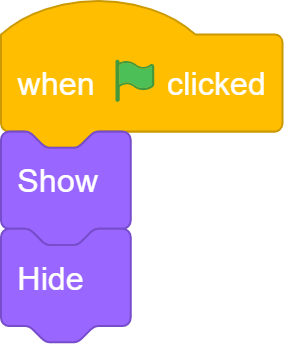
\includegraphics[width=5cm]{sequence.png} }\label{fig:sequence}}%
    \qquad
    \subfloat[Ignored subsequence]{{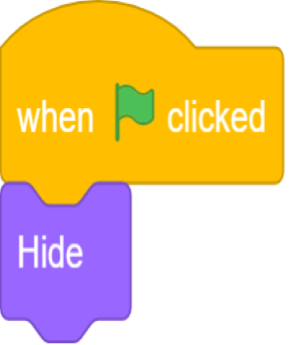
\includegraphics[width=5cm]{subsequence.png} }\label{fig:subsequence}}%
    \caption[\scratch{} block sequences]{\label{fig:sequences}\scratch{} block sequences}%
\end{figure}

If Figure~\ref{fig:sequence} would be the sequence we want to calculate the probability of, the estimation based on the \hyperref[def:markov_chain]{Markov chain} is executed by solving the Equation~\ref{eq:scratch-prob}. We are setting the \hyperref[def:gram size]{gram size} to 3 in this example. All internal probabilities are added by consulting the existing model and searching for the already calculated estimations. Therefore, the token sequence [GreenFlag, Show, Hide] can be calculated based on internal probabilities of its existing subsequences.

\begin{equation} \label{eq:scratch-prob}
\begin{aligned}
P([GreenFlag, Show, Hide]) ={} & P([GreenFlag])\cdot P([Show]|[GreenFlag]) \\
							  & \cdot P([Hide]|[GreenFlag, Show])
\end{aligned}
\end{equation}


\subsection{Smoothing of Probability Distribution}\label{subsec:smoothing}
If the analysed project is not part of the training dataset, it is important to smooth the probability distribution in order to avoid probabilities of zero. In this implementation, Add-One-Smoothing was utilized which prevents non existent sequences to be shown by adding an additional count to each n-gram.
All the counts that used to be zero will now have a count of 1, the counts of 1 will be 2, and so on. This algorithm is also called Laplace smoothing. This way there are no sequences with a probability of zero stored in the model that could affect the calculation of the sequence probabilities.

In the case of the unigram [GreenFlag], its maximum likelihood to appear in a \scratch{} project is estimated by counting the occurrences \textit{c} during the model training process and divide it through the total number of tokens \textit{N}. Therefore, the Equation~\ref{eq:likelihood} looks like this:

\begin{equation} \label{eq:likelihood}
P([GreenFlag]) ={} \frac{c}{N}
\end{equation}

Add-One Smoothing then, like the name suggests, only adds one to each count. Since there are a total of \textit{V} tokens in the model vocabulary and we added one more sighting to each one of them, we also have to adjust the denominator of the fraction accordingly. One more observation of each token means we have to increase the denominator by \textit{V}. If we apply the Math rules, the equation results in the following calculation in Equation~\ref{eq:laplace}:

\begin{equation} \label{eq:laplace}
P_{Laplace}([GreenFlag]) ={} \frac{c + 1}{N + V}
\end{equation}


\section{Bug Detection in \scratch{}}\label{sec:detection}
The specific algorithm to find bugs in \scratch{} is implemented the following way. At first, the probabilities of all sequences of the analysed project have to be calculated with help of the model like it is described in Subsection~\ref{subsec:n-grams}. After that, based on their probability the sequences are ranked and only the ones with the lowest probability get reported as potential bugs. In the next Subsection~\ref{subsec:configurations} all important parameters are set to ensure the optimal model analysis results. In Subsection~\ref{subsec:false_bugs} we found a method to minimize the amount of false positives in the reported bug set.

\subsection{Configurations}\label{subsec:configurations}
For the \scratch{} model implementation we added five parameters that have to be set accordingly in order to achieve the best evaluation results that are discussed later in Chapter~\ref{chap:evaluation}.

\paragraph{Gram Size.}
For probability calculations a \hyperref[def:markov_chain]{Markov chain} is used to get the conditional probability of a sequence using its n-1 token predecessors as context information. In this work, n-gram models with a gram size between 2 to 6 are used in order to find the optimal n for bug detection in \scratch{} projects (Section \ref{sec:gram_size}). 
\paragraph{Sequence Length.}
In the same way we used a large dataset to obtain information about the best \hyperref[def:gram_size]{gram size n}, we also analysed which length of a token sequence could be the optimal size for a good model. Finding the right length of a token sequence is evaluated in a more detailed way in Section \ref{sec:sequence_length}.
\paragraph{Reporting Size.}
In this implementation the reporting size for the big dataset model from Subsection~\ref{subsec:trainingset} is fixed at 25 reports per analysis, whereas we did not limit the report size for the small data set that  is further introduced in Subsection~\ref{subsec:bugset}. One reason for this decision was that if the reporting size is chosen too big, the risk of false positives is also increased. Furthermore, the amount of reported bugs is very small in the case of the second set because the projects as well as the model itself are not very big. If we would have restricted the amount of reported bugs even more, there would not be enough output created to analyse.  
\paragraph{Minimum Token Occurrence.}
In this bachelor's thesis \ngram{} which is only for \scratch{} analysis purposes the minimum token occurrence is chosen as one. Because of the size difference between usual Java projects compared to normal \scratch{} projects, it would not make sense to filter out any tokens. \scratch{} programmers do not have as much freedom in their implementation because of the restriction through a block-based language and usually choose a different purpose for their programs than text-based programming languages would, which leads to much smaller projects with fewer usages of specific tokens. So, the minimum token occurrence parameter would only make it harder to find low probability sequences in projects which is why we decided not to raise this threshold for the analysis.
\paragraph{Probability Threshold.}
If a sequence in the report has a probability that is higher than the given threshold, it probably is a normal token sequence that just happens to have a lower probability than the rest of the project's blocks. In this implementation, the threshold is fixed at 0.05 for the big dataset of Subsection~\ref{subsec:trainingset} and at 0.1 for the pupils' projects of Subsection~\ref{subsec:bugset}. The reason is again the size difference that would minimize the analysis output even more, if this restriction would be too low for the small project set.

\subsection{Pruning False Bugs}\label{subsec:false_bugs}
Token sequences with low probability are at the bottom of a n-gram reporting list for potential bugs. But there is always the chance that the found sequence is not actually wrong but just a very unusual or special use case in which its probability would also rank rather low. To find and filter out this kind of false bugs and reduce the candidate bug set, token sequences can only be reported when they are at the bottom of at least two ranked lists of \ngram{s} with the same \textit{gram size} but different \textit{sequence lengths}. This way, sequences are sorted out that just appear on one of these lists and the chance to report false positives gets drastically reduced. 


\section{Implementation}\label{sec:implementation}
This section explains the tool chain of our approach for \ngram{} in \scratch\ and clarifies implementation
decisions. Table~\ref{tab:ngram-params} gives an overview over the model building process in \scratch, the bug detection system, the parameters which can be adjusted, and the input and output of each step.

\begin{table}[H]
    \caption[The tool chain for n-gram bug detection in \scratch]{\label{tab:ngram-params}The tool chain for n-gram bug detection in \scratch.}

    \begin{tabular}[t]{lllll}
        \toprule
        \parbox{2cm}{Steps} & Input & Tool & \parbox{2cm}{Output\\format} & Parameters \\
        \midrule
        \vspace{10pt}
        
        \parbox[t]{2cm}{Model\\ Building} &\parbox[t]{3cm}{\scratch\ dataset,\\ \texttt{model.csv}} & \parbox[t]{2cm}{\ngramtrainer{}} & \parbox[t]{2cm}{\texttt{.csv}} & \parbox[t]{3.8cm}{\hyperref[def:gram_size]{gram size}}\\
        
        \vspace{10pt}
        
        \parbox[t]{2cm}{Bug\\ Detection} & \parbox[t]{3cm}{\scratch\ \\ bug set,\\ \texttt{model.csv},\\ \texttt{report.csv}} & \parbox[t]{2cm}{\ngrambugfinder{}} & \parbox[t]{2cm}{\texttt{.csv}} & \parbox[t]{3.8cm}{\hyperref[def:report_size]{report size},\\ \hyperref[def:gram_size]{gram size},\\ 	\hyperref[def:sequence_length]{sequence length},\\ \hyperref[def:probability_threshold]{probability \\ threshold},\\ with/without smoothing}\\ 

        \bottomrule
    \end{tabular}
\end{table}

%TODO More details?
\subsection{\tokenizer{}}\label{subsec:tokenizer}
The basis of the n-gram building process is to tokenize each project and structure it the same way. The \ngramtrainer\ as well as \ngrambugfinder\ both use \litterbox\ to create an \AST\ for a given program. The \AST\ then maps every command block to a corresponding \AST\ node. In this process every hat block is implementing the interface \texttt{Event} and all remaining command blocks are associated with the \texttt{Stmt} interface. For instance, the [Turn Right] block is represented by an object of the \texttt{TurnRight} class which implements the \texttt{Stmt} interface. A visitor then visits the \AST\ and partitions the project into its \hyperref[def:token]{tokens}.

\subsection{\ngramtrainer{}}\label{subsec:ngramtrainer}
\ngramtrainer, a feature added to \litterbox, creates a \ngram\ of a set of \scratch\ projects. The model stores a probability distribution of all token sequences that were found in the training set. It is then utilized as a foundation for bug detection in \scratch.

The model creation process consists of three steps: First, all possible sequences of tokens that can be created of the analysed training set are calculated, counted, and stored in a Map structure. Second, we go through the Map of sequences and estimate the probability of each sequence, like it is shown in Equation~\ref{eq:likelihood}, by counting the amount a sequence appeared during the n-gram calculation and dividing it by the total number of sequences. After the calculation the finished model is printed as a \textit{.csv} file and is ready for its usage in further analysis and bug detection procedures.

\subsection{\ngrambugfinder{}}\label{subsec:ngrambugfinder}
\ngrambugfinder, another extension that was added to \litterbox, continues the analysis process of the \ngramtrainer\ by using its calculated model. First of all, to find bugs in a project, the project itself is partitioned into sequences of a specific length that are also stored in a Map. Then the probability of each sequence is estimated with help of the given probability distribution of the n-gram model. The probabilities are then ranked and the sequences with the lowest score are reported as potential bugs. The final \textit{.csv} file then shows the reported sequences with their location informations and calculated probabilities.